% Created 2021-12-10 sex 16:38
% Intended LaTeX compiler: pdflatex
\documentclass[conference]{IEEEtran}
\usepackage[utf8]{inputenc}
\usepackage[T1]{fontenc}
\usepackage{graphicx}
\usepackage{longtable}
\usepackage{wrapfig}
\usepackage{rotating}
\usepackage[normalem]{ulem}
\usepackage{amsmath}
\usepackage{amssymb}
\usepackage{capt-of}
\usepackage{hyperref}
\usepackage[backend=biber,bibencoding=utf8]{biblatex}
\addbibresource{export.bib}
\usepackage{float}
\author{\IEEEauthorblockN{ Marco Antônio Ribeiro de Toledo \\ RA:\@ 11796419 } \IEEEauthorblockA{ B.Sc. in Computer Science\\ Instituto de Ciências Matemáticas e de Computação\\ University of São Paulo (USP)\\ mardt@usp.br \\ ORCiD: orcid.org/0000-0002-0484-8450}}
\IEEEpeerreviewmaketitle{}
\date{\today}
\title{\emph{Twitter Users: What Do They Know? Do They Know Things? Let's Find Out!} \\ {\LARGE Analyzing the accuracy of predictions of public approval of the government using sentiment analysis of Twitter data }}
\hypersetup{
 pdfauthor={Marco Antônio Ribeiro de Toledo},
 pdftitle={\emph{Twitter Users: What Do They Know? Do They Know Things? Let's Find Out!} \\ {\LARGE Analyzing the accuracy of predictions of public approval of the government using sentiment analysis of Twitter data }},
 pdfkeywords={social media, natural language processing, government opinion, mining},
 pdfsubject={},
 pdfcreator={Emacs 27.2 (Org mode 9.6)}, 
 pdflang={English}}
\begin{document}

\maketitle
\begin{abstract}
Social media has become more and more the unofficial ``town's square'' of our society, allowing for the sharing of opinions and discussions in this marketplace of attention. With that in mind, this paper aims to show how mining these discussions may allow for statistical inferences of its population through processes much easier than previously held standards of in person surveying, specifically in the context of political opinions, although any statistical data collected must be taken with a grain of salt due to how sensitive the accuracy of these results are to initial assumptions and data modeling.
\end{abstract}

\begin{IEEEkeywords}
data mining, social media, political analysis, prediction accuracy
\end{IEEEkeywords}

\section{Introduction}
\label{sec:orga88c40e}
The current paradigm for web content generation, the so called Web 2.0, was defined in 2005 by Tim O'Reilly as \footnote{http://radar.oreilly.com/2005/10/web-20-compact-definition.html}
\begin{quote}
\emph{[\ldots{}] the network as platform, spanning all connected devices; Web 2.0 applications [\ldots{}] [get] better the more people use it, consuming and remixing data from multiple sources, including individual users, while providing their own data and services in a form that allows remixing by others, creating network effects through an “architecture of participation,” and going beyond the page metaphor of Web 1.0 to deliver rich user experiences.}
\end{quote}
This idea of federated content creation allows the ideas expressed in these online spaces to more closely resemble the actual opinions of its constituents, encouraging users to express their personal opinions and relate to ideas expressed by peers.

The decentralized nature of this content and its ample access also allows for easy mining of huge sets of data, so considering the online content as a truthful analog for real world ideas, mining of online data asymptotically matches the real world data for the population that the users are a sample of.

With that in mind, the goal of this paper is to analyze the accuracy of online mined sentiment data, specifically in the context of government approval, compared to traditional polling, testing the hypothesis that this easily implemented method is a good real world approximation for traditionally obtained data.

\section{Related work}
\label{sec:orgea818f6}
With the widespread usage of social media, like the microblogging platform \emph{Twitter}, by the general population, its usage as a barometer for public opinion has been discussed more and more in recent years, even more so in politics, a field where accurate predictions of public opinion are essential. This resulted in ample research being done in the area, from initial work like Tumasjan et al. \cite{Tumasjan2010} in 2010 using Linguistic Inquiry and Word Count to analyze favorability rates of parties and politicians and, therefore, predict election results, to more recent and complex models like Nasrul et al. \cite{Aziz2018} in 2018 using Support Vector Machines to identify public satisfaction with government services, resulting in fairly accurate predictive models.

To support this kind of research, much has been analyzed on the ability to accurately extract sentiment data of \emph{tweets} at random, with different methods of analysis constantly being tested for their accuracy, from simple semantic scoring of corpuses as in \cite{Kumar2015} to more complex lexicon-based sentence analysis like the work done by Meduru et al. \cite{opinionTwitter}, with recent research showing that the best performing classifier considering accuracy, precision, recall and F1-score is a combination of the more complex and computationally intensive Logistic Regression and Stochastic Gradient Descent as seen in \cite{Yousaf2021}.

In the field of brazilian politics, studies have showed the accuracy of sentiment analysis models when working with \emph{tweets} from brazilian users on a portuguese corpus, as seen in \cite{Weiand2017}, and others have been conducted in the past on the accuracy of twitter content as a predictor of public opinion as seen in \cite{Oliveira2017} and \cite{Oliveira2019} giving accurate results, although running into limitations.

This approach has also been used by private companies like \emph{Arquimedes} \cite{Arquimedes2021}, with results comparable to traditional surveys conducted by companies like \emph{Vox Populi}, \emph{IBOPE} and \emph{Datafolha}, resulting in those analyses now being regularly used by many reputable sources (as seen in \cite{arquimedesMidia}).

All code used for this paper, as well as this document itself, will be available in \href{https://github.com/Ocramoi/twitter-political-analysis-accuracy}{the accompanying \emph{Github} repository.}

\subsection{Hypothesis}
\label{sec:orgf0132e1}
Taking into account previous research done in the field, our main hypothesis is that opinion data mined straight from a given social media platform (\emph{Twitter} in our case) is within margin of error of traditional polling, allowing its results to be taken as statically equivalent to the much more costly and time consuming traditional, in person, polling techniques.

This hypothesis is supported by previous work in other contexts that show the reliability of such methods in politics, as those done in Indonesia in 2018 \cite{Budiharto2018}, in the context of the french elections in 2017 \cite{Wang2017} and many others \cite{Tumasjan2010}\cite{Kassraie2017}, showing results that closely correspond to traditionally collected data. Also, other studies have already theorized on the positive impact on the popular participation in politics that could be brought to the brazilian political landscape by such data mining \cite{Oliveira2019} \cite{Oliveira2017}.

\section{Methodology}
\label{sec:org1f14c6a}
The main objective of this study is to compare the accuracy of data mining methods to the traditional polling methods on the public's opinion of the current brazilian administration, so we try to abstract the qualitative data mining classification into a quantitative identification of the public's opinion in a 3-way classification akin to the one done by IPEC in its opinion polling on the approval of the current government (as seen on its monthly press report \cite{IpecSetembro}).

Here we outline the methodological procedure for each step of this study: the data collection, extracting the relevant information from \emph{Twitter} for analysis; data preprocessing, discarding ambiguous, duplicate or otherwise irrelevant texts; sentiment analysis, extracting the sentiment data of each extracted \emph{tweet}; statistical analysis, comparing the results with ones obtained by traditional polling.
\subsection{Data collection}
\label{sec:org1c6969f}
\emph{Twitter} itself provides its own API with support for keyword based searches over any time spam with the \emph{Full-Archive search} \footnote{https://developer.twitter.com/en/docs/twitter-api/premium/search-api/quick-start/premium-full-archive},  so the information was collected running searches over relevant keywords for our context: \emph{'Bolsonaro', 'governo', 'presidente'}, \emph{'país'} and \emph{'mito'} within the analyzed period for the analysis. The time spent in this step is directly related to the usage of the Twitter API and its search quota for the given access level, being the bulk of the processing time.
\subsection{Data preprocessing}
\label{sec:org65554cd}
For a more representative data set, focusing on reducing inconsistencies, redundancies and misleading information in the data, we had to, before starting the sentiment analysis, clear the data set removing:
\begin{itemize}
\item \emph{Tweets} containing URLs, which may indicate an ambiguous text (differentiating if the sentiment expressed refers to the contents of the URL or the subject would require further investigating), detected with regular expressions
\item Repeated, non retweeted text, which may indicate content by spam bots, detected by keeping a set of unique tweets
\item User handles, anonymizing the data for publishing, replaced using regular expressions
\end{itemize}
\subsection{Sentiment analysis}
\label{sec:orge137b4a}
Once we had the striped text for each \emph{tweet} and its related keyword from whose search the data was extracted, we could analyze the sentiment of each instance and tally them to the overall sentiment of each keyword. Due to the limitations in the scope of this paper, the sentiment mining was done using LeIA \cite{Almeida2018} a brazilian-portuguese \emph{fork} of the lexicon-based sentiment analysis tool VADER \cite{Hutto2014}. The original tool has great accuracy for this kind of analysis considering its 0.96 F1 score on 3-class accuracy for a corpus of \emph{tweets} while also maintaining good performance due to its lexical nature.
\subsection{Statistical analysis}
\label{sec:orgb42949f}
We propose then taking the harmonic mean of these values as an abstraction of the overall opinion on the current brazilian administration, which can be compared to IPEC's public opinion poll on administrative/political subjects (\emph{PESQUISA DE OPINIÃO PÚBLICA SOBRE ASSUNTOS POLÍTICOS/ADMINISTRATIVOS}) \cite{IpecPesquisas} in the respective time period, ideally being within its margin of error of 2 percentage points.

\begin{figure}[H]
\centering
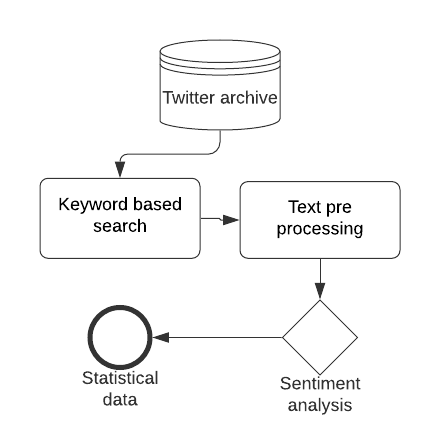
\includegraphics[width=\linewidth]{./Metodologia.png}
\caption{\label{fig:dataflow}Data analysis flowchart.}
\end{figure}

\section{Results}
\label{sec:orgaacc6b8}
The latest compiled public opinion poll on the brazilian government done by IPEC dated June 2021 (from 06-17-2021 to 06-21-2021) \cite{AvaliacaoGovernoIPEC} was used as reference for the analysis, with the \emph{Twitter} data being collected from the same span of time. The underlying reference question for the classification was \emph{Do you personally approve or disapprove of the way} President Jair Bolsonaro \emph{is governing Brazil?}, with the following data (0.95 confidence with a margin of error of 0.02):

\begin{center}
\begin{tabular}{lllll}
 & Approves & Disapproves & Other* & Total\\
\hline
Count & 601 & 1321 & 80 & 2002\\
Percentage & 30\% & 66\% & 4\% & 100\%\\
\end{tabular}
\end{center}
\emph{* either 'doesn't know' or 'didn't answer'.}

\begin{figure}[H]
\centering
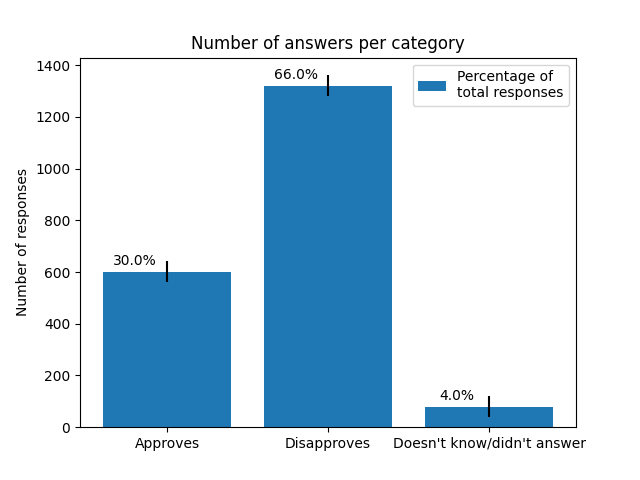
\includegraphics[width=\linewidth]{./ValsIPEC.png}
\caption{\label{fig:polls}Polling results.}
\end{figure}

\begin{figure}[H]
\centering
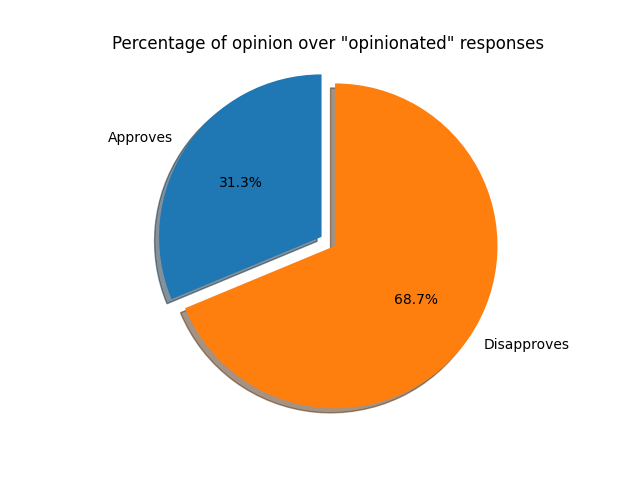
\includegraphics[width=\linewidth]{./piePoll.png}
\caption{\label{fig:nonneutral}Overral classification of binary responses.}
\end{figure}

Due to limitations of the free tier \emph{Twitter} API, only 1750 \emph{tweets} were collected using the archive search over the corresponding time span, which resulted in a data set of \(n = 1524\) usable \emph{tweets} after the post processing that were later classified using a custom fork of LeIA \footnote{https://github.com/Ocramoi/LeIA}, adapting some features for this specific analysis (this process is also explained in the documentation for the accompanying code).

The classification of the overall sentiment of a \emph{tweet} was done using the compound score for the analyzed text. As per the original documentation for the tool, \emph{tweets} with a compound score of over 0.05 were classified as positive, with \(m_{positive}\) total tweets, those with a scores lower than -0.05 were classified as negative, with \(m_{negative}\) total tweets, and the rest were included as ``neutral'', totaling \(m_{neutral}\) tweets. The percentage of \emph{tweets} in each category was taken as an estimator for the overall opinion of the population as such:
$$ \hat{p}_{approves} = \frac{m_{positive}}{n} $$
$$ \hat{p}_{disapproves} = \frac{m_{negative}}{n} $$
$$ \hat{p}_{other} = \frac{m_{neutral}}{n} $$
Also, due to the lack of precision in keyword based mining, resulting in an elevated number of neutral tweets, the ratio of approval within those with a binary answer (approves/disapproves) was also estimated, as such:
$$ \hat{p}_{ratio} = \frac{m_{positive}}{n - m_{neutral}} $$

The raw data collected was as follows:
\begin{center}
\begin{tabular}{lllll}
 & Positive & Negative & Neutral & Total\\
\hline
Count & 388 & 836 & 300 & 1524\\
Percentage & 25\% & 55\% & 20\% & 100\%\\
\end{tabular}
\end{center}

\begin{figure}[H]
\centering
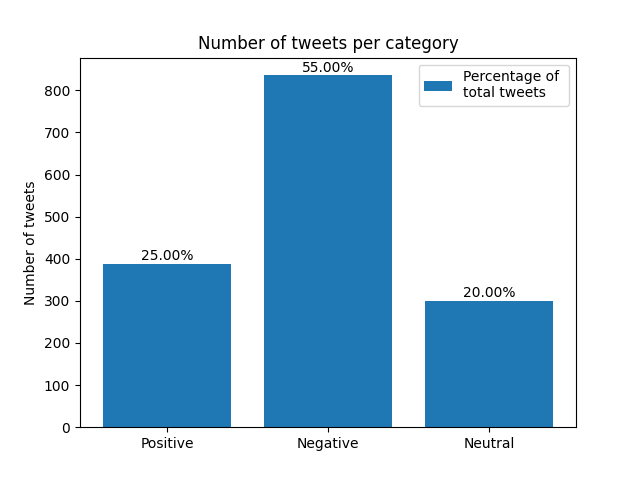
\includegraphics[width=\linewidth]{./ValsTwitter.png}
\caption{\label{fig:mined}Mining results.}
\end{figure}

\begin{figure}[H]
\centering
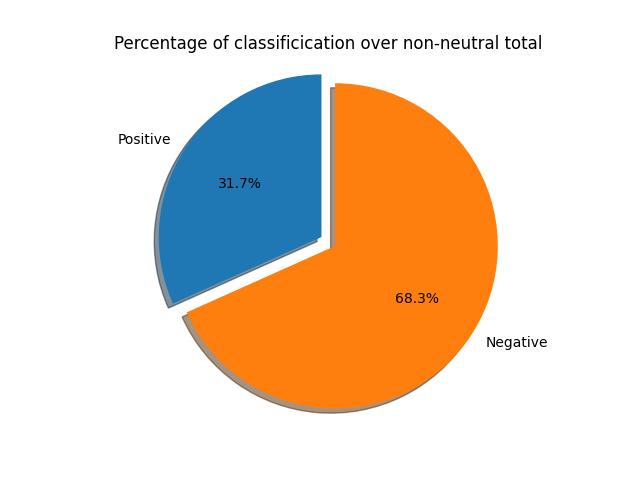
\includegraphics[width=\linewidth]{./pieTweet.png}
\caption{\label{fig:nonneutral}Overral classification of non-neutral tweets.}
\end{figure}

From which we can calculate our biases as follows
$$ V(\hat{p}_{approves}) = \frac{388}{1524} - 0.30 \approx -0.045 $$
$$ V(\hat{p}_{disapproves}) = \frac{836}{1524} - 0.66 \approx -0.111 $$
$$ V(\hat{p}_{other}) = \frac{300}{1524} - 0.04 \approx 0.157 $$
$$ V(\hat{p}_{ratio}) = \frac{388}{1524 - 300} - \frac{601}{2002 - 80} \approx 0.004 $$

This shows a strong bias in favor of neutral responses, with the total number of \emph{tweets} in each category being a weak indicator for the overall population taking the polling as a standard, with values well over the margin of error. However, the estimated ratio of positive responses over the total number of ``opinionated'' ones does describe the sample fairly well, reinforcing the idea that the naive data mining over the \emph{tweets} with only keywords tends to over represent neutral responses.

\section{Discussion and future work}
\label{sec:org1080803}
The generated estimates show that when well modeled, estimates over social media mined data may give us true-to-life results, allowing for an easier, cheaper and faster way of assessing sentiment data over a online-represented population, like the Brazilian demographic in our example. However, it also shows how sensitive the accuracy of this predictions is to the definition of initial assumptions and statistical models.

In the field of political analysis, this kind of data is of utmost importance for everyday analysis involving public assessments, for example, political campaigns, policy satisfaction surveying, voting intention, etc. Considering the price of traditional in person polling, running anywhere from R\textdollar 18.95 to R\textdollar 115.50 per person \footnote{https://www.moneytimes.com.br/quanto-custam-as-pesquisas-eleitorais-veja-as-mais-caras/}, the near gratuity of a data mining method like the one presented in this paper (safe some men/hours of initial setup and statistical work) expands greatly the accessibility of such data, showing the importance and utility of more research in the area.

Future work in this question could tackle some of the short comings of the methods used, from the small sample size, inflexibility of the lexicon matching (not accepting acronym expansion, misspellings, and other important features, for example) or lackluster statistical analysis. Other methods of sentiment analysis should surely be tested, from expanded lexicon based ones to models using supervised machine learning like a Support Vector Machine, or, as suggested by Yousaf, et. al \cite{Yousaf2021}, Stochastic Gradient Descent/Linear Regression, over pre classified \emph{Twitter} data, like the reliable \emph{TweetSentBR} \cite{Brum2017}. The manual classification of \emph{tweets} for the classifiers could yield even better results for more recent analyses, making sure to base estimations on up to date models, although this would grow considerably the scope and costs of such analysis.

\printbibliography{}
\end{document}
